\chapter{Análisis de Resultados}

\lettrine[lines=1]{U}n método para investigar que sucedió con la galaxia UGC11680, es interpretar
la información que nos provee su  historia de ensamblaje de masa estelar, analizando los datos que se obtienen del mapa $SFH$, ya que esto nos dará claves para saber si su apagado fue un proceso de dentro hacia afuera ó viceversa. Para esto, nos interesará saber si la historia de formación estelar se parece a algún tipo de historia  promediada de otras galaxias o tipos de galaxias.

\bigskip

\noindent Así mismo,  podemos comparar con promedios de diferentes tipos de galaxias, dada la característica principal de la galaxia UGC11680: con el promedio de los AGNs tipo dos, y con promedios en categorías color-masa. Estos promedios se contrastan con la galaxia que estamos estudiando y ver en donde ajusta o difieren.
Esto tiene implicaciones inmediatas: en la literatura astronómica no existe esta clase de comparaciones, por lo que en si misma, ofrece
una metodología nueva gracias a la espectroscopía de campo integral y sus mapas  $SFH(t,R)$

\section{Los Datos y sus Promedios}

\noindent Se utilizaron 574 mapas $SFHs$ de la muestra de \textbf{CALIFA} y se dividieron en los siguientes grupos:

\begin{itemize}

  \item En 24 AGNs de tipo 2 de la muestra, sin importar su morfología.

  \item Los 574 SFH divididos por categorías de color-masa, para simular el diagrama color-masa de galaxias, pero con mapas $SFHs$. Esta clasificación es de suma importancia ya que estudios anteriores muestran que la masa es fundamental para determinar el tipo de crecimiento en galaxias.

\end{itemize}

\noindent Detallando más las categorías, se dividieron las 574 $SFH$ de cada galaxia en cuatro bines de masa. Una vez dividido, a su vez esas categorías se dividieron por color. El número de galaxias en cada categoría se muestran en la Tabla \ref{tab_CMD}. Para cada división, se utilizó su mapa $SFH(t,R)$.

\bigskip



\noindent Es importante señalar que excluimos los bines de menor masa y color por tener un sólo objeto y por lo tanto no tener importancia estadística. Así mismo, la zona de las galaxias más rojas y masivas ($\sim 10^{11.5} M_{\odot}$) contiene solo 6 mapas $SFH$, pero lo mantendremos por la importancia comparativa  con la galaxia de estudio. Por último, a pesar de que separamos los AGNs para su análisis, estos mismos fueron incluidos en su categoría color-masa correspondiente. UGC11680 se excluyó del promedio de los AGNS, pero se incluyó en su categoría correspondiente en color-masa ($3 \le g-r \le 4$ ; $11 \le M_{\odot} \le 12$)
.

\begin{figure}
  \centering
    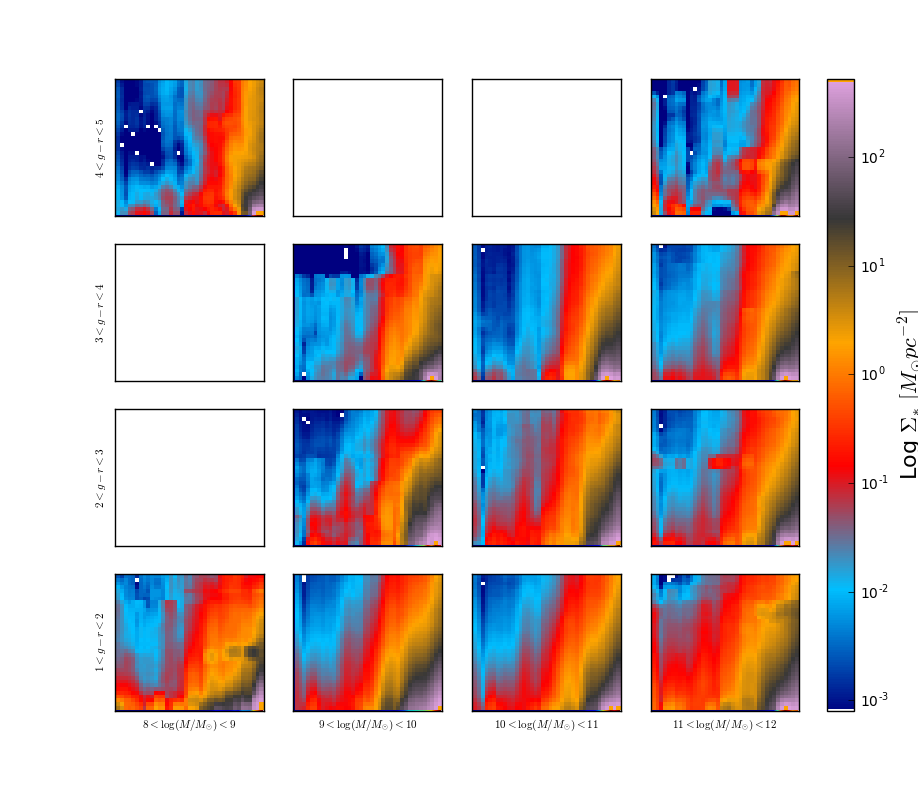
\includegraphics[scale=0.6]{cmd_sfh.png}
  \caption[Diagrama Color-Masa para la muestra de CALIFA]{Diagrama Color-Masa  para las $SFH(t,R)$ pertenecientes a su intervalo correspondiente.
           Cada $SFH(t,R)$ de la muestra de  \textbf{CALIFA} individual fue promediado con todos los de su categoría,
           por lo que cada una de ellas muestra un promedio para el intervalo de color-masa correspondiente. En la esquina superior izquierda, esta el mapa de UGC11680, por comparación.La cantidad de galaxias para cada categoría están dados en la tabla \ref{tab_CMD}. Las escalas temporales y radiales son las mismas que se dieron para mapas de galaxias individuales.Nótese el ensamblaje más grande para galaxias más masivas, además del lento ensamblaje de las galaxias más ligeras, además del apagado de UG11680, mas notorio debido al escalamiento.}
  \label{CMD}
\end{figure}



\begin{table}[!ht]
\centering
\begin{tabular}{||c | c | c | c | c||}
\hline
\hline
Color  / $\log$ Masa & $8< M_{\odot} < 9$ & $9< M_{\odot}< 10$ & $10< M_{\odot}< 11$ & $11< M_{\odot}< 12$ \\
\hline
\hline
$0< (g-r)<1$ & 1 & 1  & -- & -- \\

$1< (g-r)<2$ & 8 & 15 & 18 & 28 \\

$2.< (g-r)<3$ & -- & 63 & 114 & 67 \\

$3< (g-r)<4$ & -- & 87 & 70 & 96\\

$4< (g-r)<5$ & -- & -- &-- & 6\\
\hline
\hline
\end{tabular}
\caption{Disposición de las galaxias de la muestra de acuerdo a su color y masa. Las partes vacías pertenecen a categorías que no contenían objetos en la muestra.}
\label{tab_CMD}
\end{table}

\section{Promedios de los $SFH(t,R)$}

 El promedio por categoría $SFH_{cat}$ está dado por la definición clásica


\begin{equation}
\left<SFH_{cat}(t,R)\right> = \frac{1}{m}\sum_{i=1}^{m} SFH_{i} (t,R)
\end{equation}

\begin{figure}[htbp]
\centering
\subfigure[UGC11680]{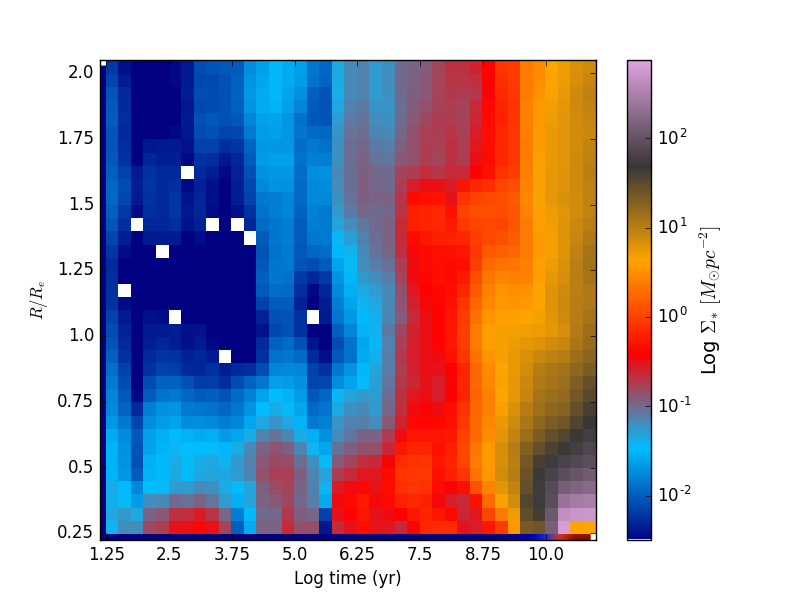
\includegraphics[width=80mm]{sfh_map_ugc11680.png}}
\subfigure[Todos los AGNs Promediados]{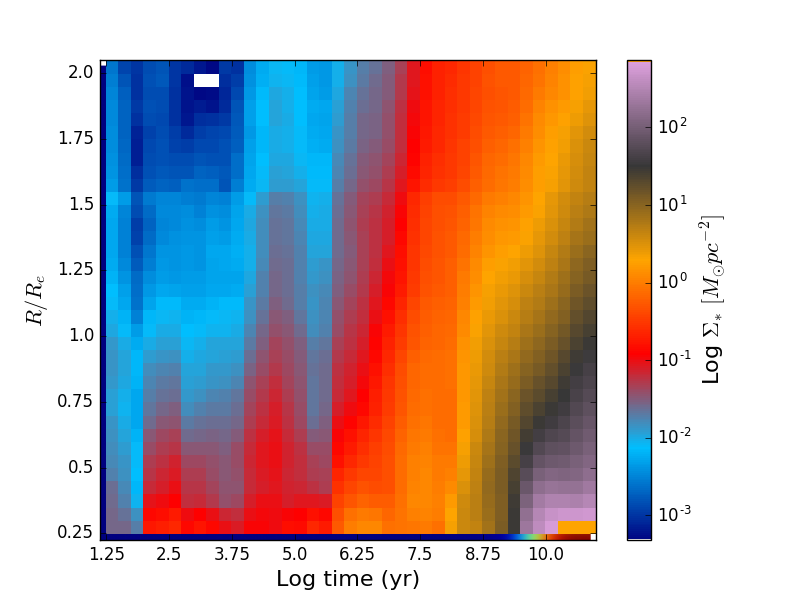
\includegraphics[width=80mm]{all_agns_mgh.png}}
\caption[Historias de Formación estelar, para UGC11680 y AGNs]{Historias de Formación estelar, para UGC11680  y AGNs tipo 2. Comparando cada mapa, ya es clara la diferencia entre UGC11680 y este promedio, ya que UGC11680 muestra un abrupto cambio en su densidad de masa estelar, en forma de corte diagonal, que parte de su centro y que comienza en $\sim$ 10 Gyrs. Nótese también en ensamblaje de dentro hacia afuera de los 3 mapas.}
\label{all_agns_sfh}
\end{figure}


\noindent Entonces, el $SFH_{cat}(t,R)$ es la suma  de $i-$ objetos en cada categoría.
Por ejemplo, para el caso del grupo de AGNs, $cat$= AGNs y m=24 el número de $SFHs$
en este grupo. Análogamente, consideramos cada categoría en la selección de galaxias por color-masa.
El paso siguiente seria entonces definir parámetros que nos den información
para comparar  el $SFH_{cat}$ para los diferentes promedios con la galaxia UGC11680. Estos promedios, junto con la $SFH$ de UGC11680 se muestran en las Figuras \ref{CMD} y \ref{all_agns_sfh}.
\bigskip

\noindent En la Figura \ref{CMD} podemos apreciar  como la masa determina en gran medida la rapidez de ensamblaje de la densidad estelar (e.g., \citep{perez2013}; \citep{perezg2008}) ;({\color{red} Ibarra-Medel, et al. Submitted }) . El mapa  $SFH$ de la galaxia UGC11680 se colocó en la esquina superior izquierda para su comparación y referencia. Notamos que para galaxias  más masivas, el ensamblaje de masa  es más rápido. También observamos que las galaxias menos masivas  es notorio que en promedio todavía siguen formando estrellas a edades actuales. Ahora, en la Figura \ref{all_agns_sfh} vemos que los AGNs carecen del corte diagonal que existe en el mapa $SFH$ de UGC11680, así como las diferentes densidades que muestra la espiral roja, sobre todo en las partes medias y externas. Nótese igualmente que aunque los AGNs no muestran ese corte tan notorio como UGC11680, si muestran una evolución temporal de densidad de masa estelar más abrupto que UGC11680.



\section{Parámetros Analizados}

En esta sección obtendremos parámetros básicos para el análisis de $SFHs$ ya sean individuales o de promedios.
Estos parámetros ya han sido analizados anteriormente en la literatura sobre galaxias
espacialmente resueltas, tal como en \citet{cid2013_1} \cite{perez2013} y \citet{gonzalezdelgado2016} {\color{red} Ibarra-Medel, et al. (Submitted) }. En nuestro caso, estos parámetros son importantes ya que nos dirán si la galaxia de nuestro estudio creció de dentro hacia afuera y si detuvo su formación estelar. De esta forma, al compararla con los promedios sabremos si su comportamiento es atípico para galaxias con sus características o es algo común en el grupo seleccionado.


\subsection{Perfil Radial de Densidad de Masa Estelar ($PR \Sigma_{*}$) }

A partir del mapa $SFH$ también podemos calcular la densidad de masa acumulada radialmente a cualquier tiempo/edad dada su distancia radial normalizada al radio efectivo ($R/R_e$). Para esto, definimos su perfil radial de densidad de masa estelar acumulada $PR \Sigma_{*}$ como

\begin{equation}
PR \Sigma_{*}= \sum_{t=1}^{n_t} SFH(t,R)
\end{equation}



\noindent Donde $n_{t}$ es la dimension temporal de la imagen. Este perfil nos da información de como se acumuló masa a diferentes radios, desde las partes centrales hasta las afueras. Así mismo, se podría integrar la formula a todo tiempo y sacar un $PR \Sigma_{*}$ promedio actual para la galaxia en cuestión. Los valores esperados de esta acumulación de masa serían gradientes con pendiente negativa conforme nos alejaremos de las zonas centrales y en el caso de una disminución de acumulación de masa estelar el cambio sería a un gradiente de pendiente positiva ó plana. El resultado se muestra en la Figura \ref{perfil_radial}. Se dividió en 4 épocas cosmológicas, para una comparación más sencilla.

\bigskip

\noindent Observamos que los AGNs tipo 2 muestran la caída típica (indicador de una formación dentro-fuera) desde las zonas centrales a las afueras de estas galaxias. Esto se repite para cada época cosmológica seleccionada. Esta acumulación de masa es mayor en las partes centrales que en las partes medias, así como las afueras de estas. La acumulación de masa es mayor de dentro hacia afuera. Ahora, para la espiral roja notamos que a épocas $\sim$ 14Gyrs tiene una acumulación de masa mayor en las partes centrales que va cayendo conforme se aproxima a sus zonas externas. Sin embargo, esta acumulación cambia su gradiente en las partes centrales tanto en $\sim 12$ Gyrs como en $\sim$ 8 Gyrs. Esto nos indica que UGC11680 dejó de acumular masa en esas zonas para después tener la caída típica hacia las afueras que vuelve a cambiar en las zonas medias, para caer finalmente en las partes externas. Estos cambios se notan en $z \sim 0$ en la parte media. Esto cambios de pendiente implican que la galaxia roja efectivamente tiene a diferentes épocas momentos en que  ensambla masa, pero vuelve a tener caídas de acumulación con respecto a los promedios. Algo parece regular la acumulación de masa, y que es un proceso que comienza en las partes centrales.






\begin{figure}[htbp]
\centering
\subfigure[UGC11680]{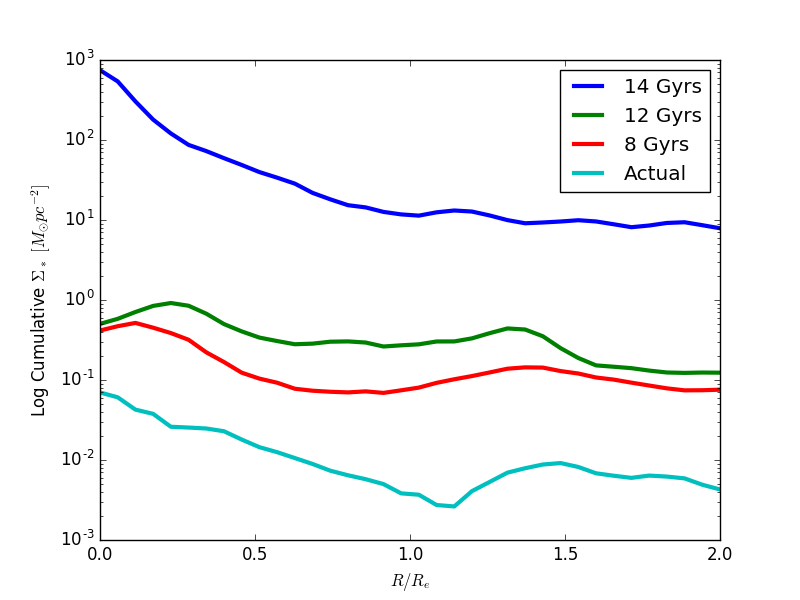
\includegraphics[width=60mm]{ugc11680_pr.png}}
\subfigure[AGNs]{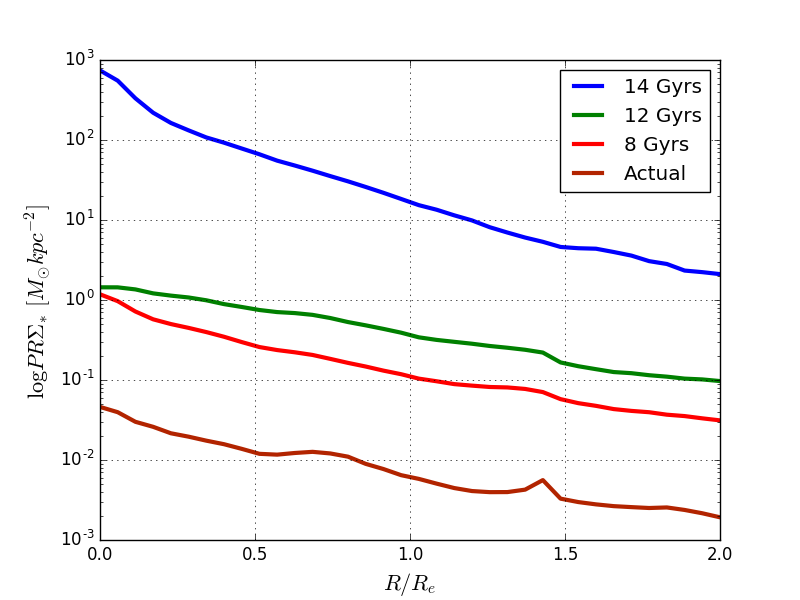
\includegraphics[width=60mm]{radial_all_agns.png}}
\caption[Perfil radial de masa estelar cumulativa de UGC11680 y AGNs]{Perfil Radial de densidad de masa superficial cumulativa de UGC11680 y los AGNs tipo 2. Cada color muestra diferentes épocas, escogidas para una mejor disposición visual. El aplanamiento en el gradiente de densidad radial para la espiral roja en épocas intermedias, mientras que los AGNs mantienen un gradiente una densidad de masa estelar casi constante en su historia de formación estelar}
\label{perfil_radial}
\end{figure}



\subsection{Historia de Crecimiento de Masa ($HCM(t)$)}

\begin{figure}[htbp]
\centering
\subfigure[UGC11680]{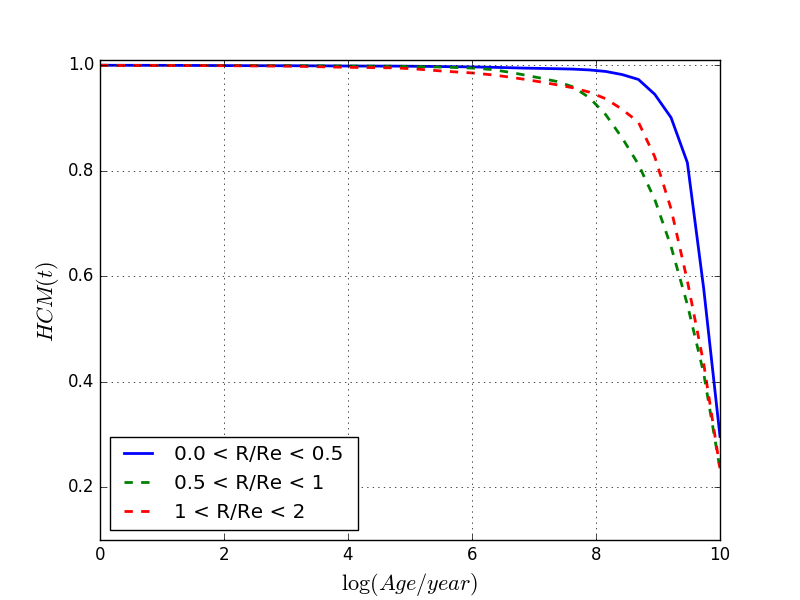
\includegraphics[width=60mm]{ugc11680_mgh.png}}
\subfigure[AGNs]{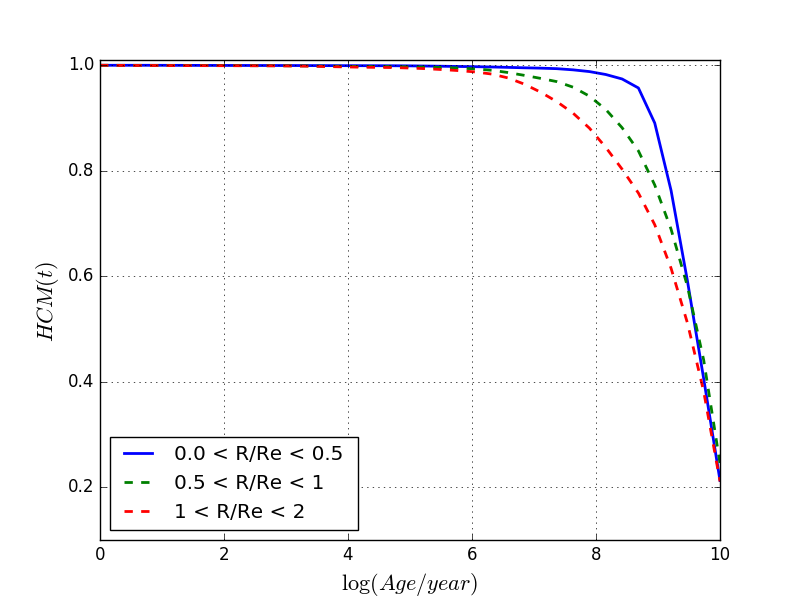
\includegraphics[width=60mm]{all_agns_mgh_log.png}}
\caption[MGHs para UGC11680 y AGNs]{Gráfica de ensamblaje de masa cumulativa de UGC11680 y los AGNs tipo 2. La línea azul corresponde a la parte central medida por su radio efectivo, la verde a la parte media y la roja a las afueras, normalizadas a la masa actual. Aunque no es concluyente para el apagado, si lo es para demostrar que UGC11680 y los AGNs ensamblaron su masa de dentro hacia afuera.}
\label{ensamblaje_log}
\end{figure}

\bigskip

\noindent Siguiendo la misma línea de razonamiento,  tomamos el mapa $SFH(t,R)$ para ahora ver el crecimiento acumulativo de la masa estelar $M_{*}$. Esto nos indicará si el crecimiento es de dentro hacia afuera a escala temporal (a diferencia del parámetro de la sección anterior, que fue dependiente del radio) o viceversa, así como el apagado, (si es que existiera) en su formación estelar. Definimos entonces la historia de crecimiento en masa como la masa relativa al total $M(t)/M_{T}$. Este parámetro normalizado contiene 39 intervalos de tiempo, por lo que obtenemos la $HCM(t)$ o historia cumulativa de masa como

\begin{equation}
HCM(t)= \frac{1}{M(T)} \sum_{R=1}^{n_R} SFH(t,R) + M(t-1)
\end{equation}

\noindent Donde

\begin{equation}
M_{T}= \sum_{R=1}^{n_R} \sum_{t=1}^{n_t} SFH(t,R)
\end{equation}

\bigskip

\noindent  $HCM(t)$  es la masa estelar relativa acumulada al tiempo $t$ y donde $n_t$ y $n_R$ son las dimensiones temporal y espacial, respectivamente. Por lo tanto, esta definición cuantifica la cantidad de masa estelar que se acumula durante la evolución de la galaxia. De esta forma podemos obtener diferentes historias de acumulación masa a lo largo de la distribución radial, simplemente integrando sobre diferentes regiones determinadas por el radio efectivo. Como nuestros mapas tienen 36 intervalos de radio normalizado, integraremos en 3 partes de 12 intervalos cada uno, a menos de que se especifique lo contrario. A diferencia del perfil radial, esta gráfica nos indica la acumulación en el tiempo, comparada con su masa final a diferentes radios efectivos. Un perfil con pendiente mas inclinada nos dará las zonas en donde ensambló primero su masa. El resultado se muestra en la Figura \ref{ensamblaje_log}.

\bigskip

\noindent Observamos que en los dos casos ya podemos decir que para los AGNs y UGC11680 el crecimiento en todos los casos es de dentro hacia afuera dado que la línea azul que representa la parte central, tiene la pendiente más pronunciada, (Al menos desde los últimos 3-4 Gyrs) seguido por sus partes medias y terminando en sus afueras, algo observado por \citet{perez2013} y por {\color{red} Ibarra-Medel, et al. (Submitted) }, por ejemplo. Obsérvese también que en los dos casos, el ensamblaje de su masa final termina en $\sim$ 1 Myr. Sin embargo, la bondad de la escala logarítmica-temporal para determinar el crecimiento dentro-fuera, carece de detalle para saber si existió un apagado en su acumulación masa. Para eso simplemente cambiamos el tiempo a escala lineal, este cambio se muestra en la Figura \ref{ensamblaje_lineal}.


\begin{figure}[htbp]
\centering
\subfigure[UGC11680]{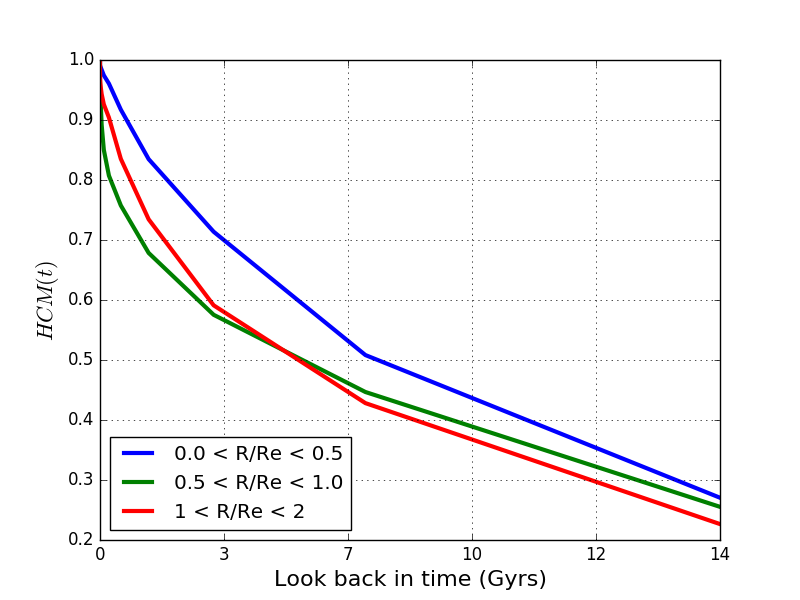
\includegraphics[width=60mm]{ugc11680_mgh_lineal.png}}
\subfigure[AGNs]{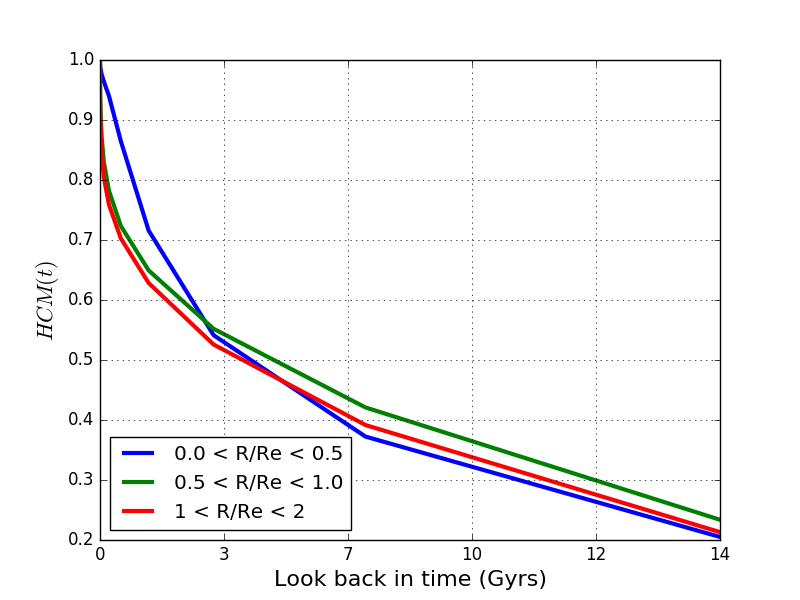
\includegraphics[width=60mm]{all_agns_mgh_lineal.png}}
\caption[Historia de Crecimiento de Masa con tiempo lineal, UGC11680 y AGNs tipo 2]{Gráfica de Ensamblaje de masa cumulativa de UGC11680 y AGNs tipo 2, con los mismos colores que la figura \ref{ensamblaje_log} pero hora a una escala temporal lineal. Nótese que ya es evidente el apagado en formación estelar comparado con los otros promedios. Esta gráfica y la figura \ref{ensamblaje_log} ya son muestran del apagado de dentro hacia afuera de UGC11680.}
\label{ensamblaje_lineal}
\end{figure}



\noindent Estas figuras ya muestran diferentes resultados según se observen los promedios ó la galaxia UGC11680. Para esta última vemos que en todo momento, la galaxia ensambla su masa desde el centro hacia afuera, es decir, un crecimiento ``dentro-fuera''. Sin embargo algo sucede en épocas $\sim$ 6 Gyrs: el ensamblaje se vuelve mas lento con respecto a las afueras, hasta que finalmente se ensambla primero la masa estelar en las afueras de la galaxia para finalmente terminar con las partes medias. Parece ser entonces que la zona media detiene (pero no completamente) su ensamblaje de masa estelar.En el caso de UGC11680, esta ensambla el 50\% de su masa estelar a $\sim$ 4 Gyrs y finalmente el promedio de los AGNs a  $\sim$ 3 Gyrs.

\bigskip

\noindent Podemos decir entonces que la galaxia espiral roja, en todo momento, ensambla su masa estelar desde dentro hacia afuera, pero las partes centrales pierden intensidad en la acumulación de masa frente a las partes externas hasta que  estas ensamblan primero su masa estelar antes que las partes medias. Esto junto con el perfil radial de densidad de masa analizado en la sección anterior, así como el mapa $SFH$ nos dicen que el ensamblaje de masa estelar de UGC11680 muestra que las zonas tanto centrales como medias detuvieron parcialmente su ensamblaje, aún frente los AGNs promediados. En todos los casos, el crecimiento es de dentro hacia fuera en ciertas épocas cosmológicas.



\subsection{Distribución Radial de la Densidad Superficial de la Tasa de Formación Estelar}

\begin{figure}[htbp]
\centering
\subfigure[UGC11680]{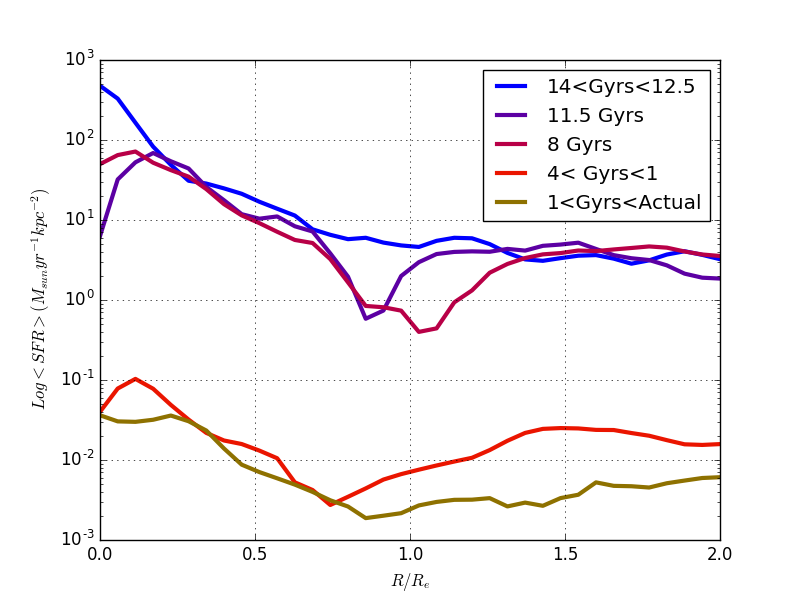
\includegraphics[width=70mm]{ugc11680_sfr.png}}
\subfigure[AGNs]{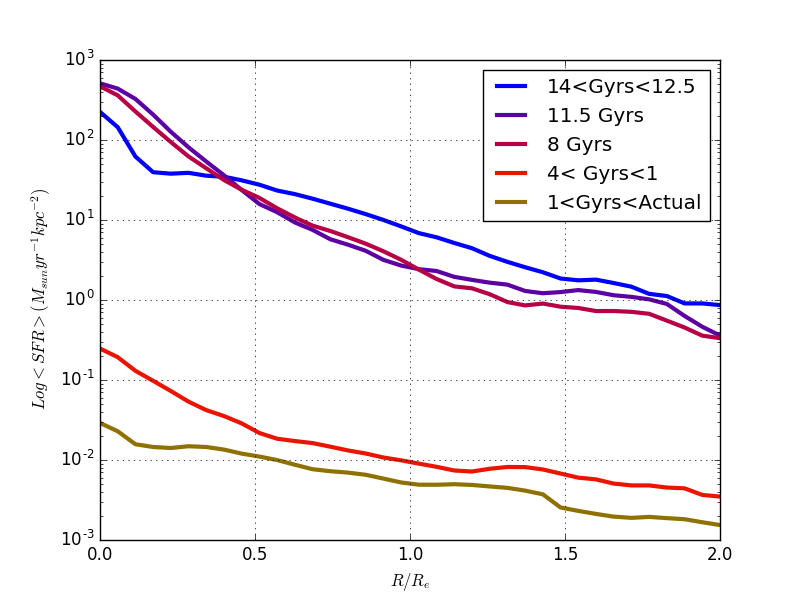
\includegraphics[width=70mm]{all_agn_sfr.png}}
\caption[Tasas De formación Estelar Radiales]{Distribución Radial de la densidad de formación estelar a diferentes edades para la galaxia de estudio, UGC11680  y los AGNs.}
\label{sfr}
\end{figure}


\noindent Como se mencionó anteriormente, podemos obtener la tasa de formación estelar a cada edad cosmológica ó a cada tiempo con ayuda de el mapa $SFH$. Esta se calcula como el cambio en masa estelar con respecto al tiempo, es decir

\begin{equation}
SFR(R)= \frac{\Delta SFH(t,R)}{\Delta t}
\end{equation}


\noindent El resultado de esta ecuación para distintos tiempos se muestra en la Figura \ref{sfr}. La interpretación de la gráfica es muy parecida a la de perfil radial, donde igualmente se consideran diferentes épocas cosmológicas para mayor interpretación visual, solo que para este caso hablamos de una tasa de formación y no una acumulación de masa estelar. Así, la $SFR$ temporal nos corrobora lo obtenido con los otros parámetros de acumulación de masa, tanto radial como temporal-porcentual: UGC11680 detuvo su formación estelar comenzando en las zonas centrales (El cambio a pendiente negativa). Sin embargo, la $SFR$ temporal nos da un resultado mas sutil: este apagado no es algo constante y sostenido, sino que aparece y desaparece dependiendo de la época cosmológica considerada. Esto implica que más que un apagado constante, la parte central aparecen eventos secuenciales de apagado y encendido, en lugar de detener completamente la formación estelar en el caso de UGC11680, lo que no se aprecia con el mapa $SFH$ de esta galaxia. Nótese además que a épocas cosmológicas actuales, prácticamente en todos los grupos de galaxias, la producción de estrellas es baja, y que en todos los casos la caída de la SFR es pronunciada en las partes externas, aunque UGC11680 tiene ligeros brotes de formación en las partes medias que ya habían notado en los otros parámetros así como en la inspección visual.

\bigskip

\noindent Podemos decir que estos tres análisis combinados, ya nos dicen que el comportamiento de UGC11680 es atípico con respecto a los promedios utilizados. los perfiles radiales nos dicen que efectivamente, se detuvo la formación estelar en las partes centrales, aunque no de manera sostenida. El perfil temporal nos dice que este proceso es dentro hacia afuera. Es decir. la masa y el AGN son algo fundamental en este proceso. Ahora podemos preguntarnos, ¿Que tan atípico es con respecto a los promedios que se utilizaron? Esto nos permitirá saber si la $SFH$ encaja en con algún otro promedio de galaxias y por lo tanto determinar a que grupo de galaxias pertenece su historia de formación estelar.




\section{Comparación y ajuste usando la distribución $\chi^{2}_{\nu}$}

Una vez analizados los parámetros para la galaxia UGC11680 y los diferentes promedios, podemos
comparar el $SFH$ de  UGC11680  con los demás $SFH's$ promediados por categorías. Esto nos dirá estadísticamente a que grupo de los clasificados con anterioridad encaja mejor esta galaxia, en función de su mapa $SFH$. Esto es importante ya que comparamos historias de formación estelar, además de que esto nos dirá (en promedio) como ha sido la evolución de ensamblaje estelar de las demás de la muestra.

\bigskip


\noindent Entonces para poder hacer una comparación cuantitativa entre $SFHs$ utilizamos el parámetro $\chi^{2}_{\nu}$ que representa un valor $\chi^{2}$ reducido por el número de grados de libertad. Para nuestro caso, la dimensión de la imagen determinará estos grados de libertad con los que se va a dividir la $\chi^{2}$. Como la dimensión de nuestros mapas en el espacio radial es 36 (dado por el radio normalizado al radio efectivo) mientras que en el espacio temporal es 39 (dados por las SSPs), los grados de libertad serían  $36 \times 39$. De esta forma, definimos la $\chi^{2}_{\nu}$ para cada galaxia con respecto a la categoría a la que pertenecen como




\begin{figure}[htbp]
\centering
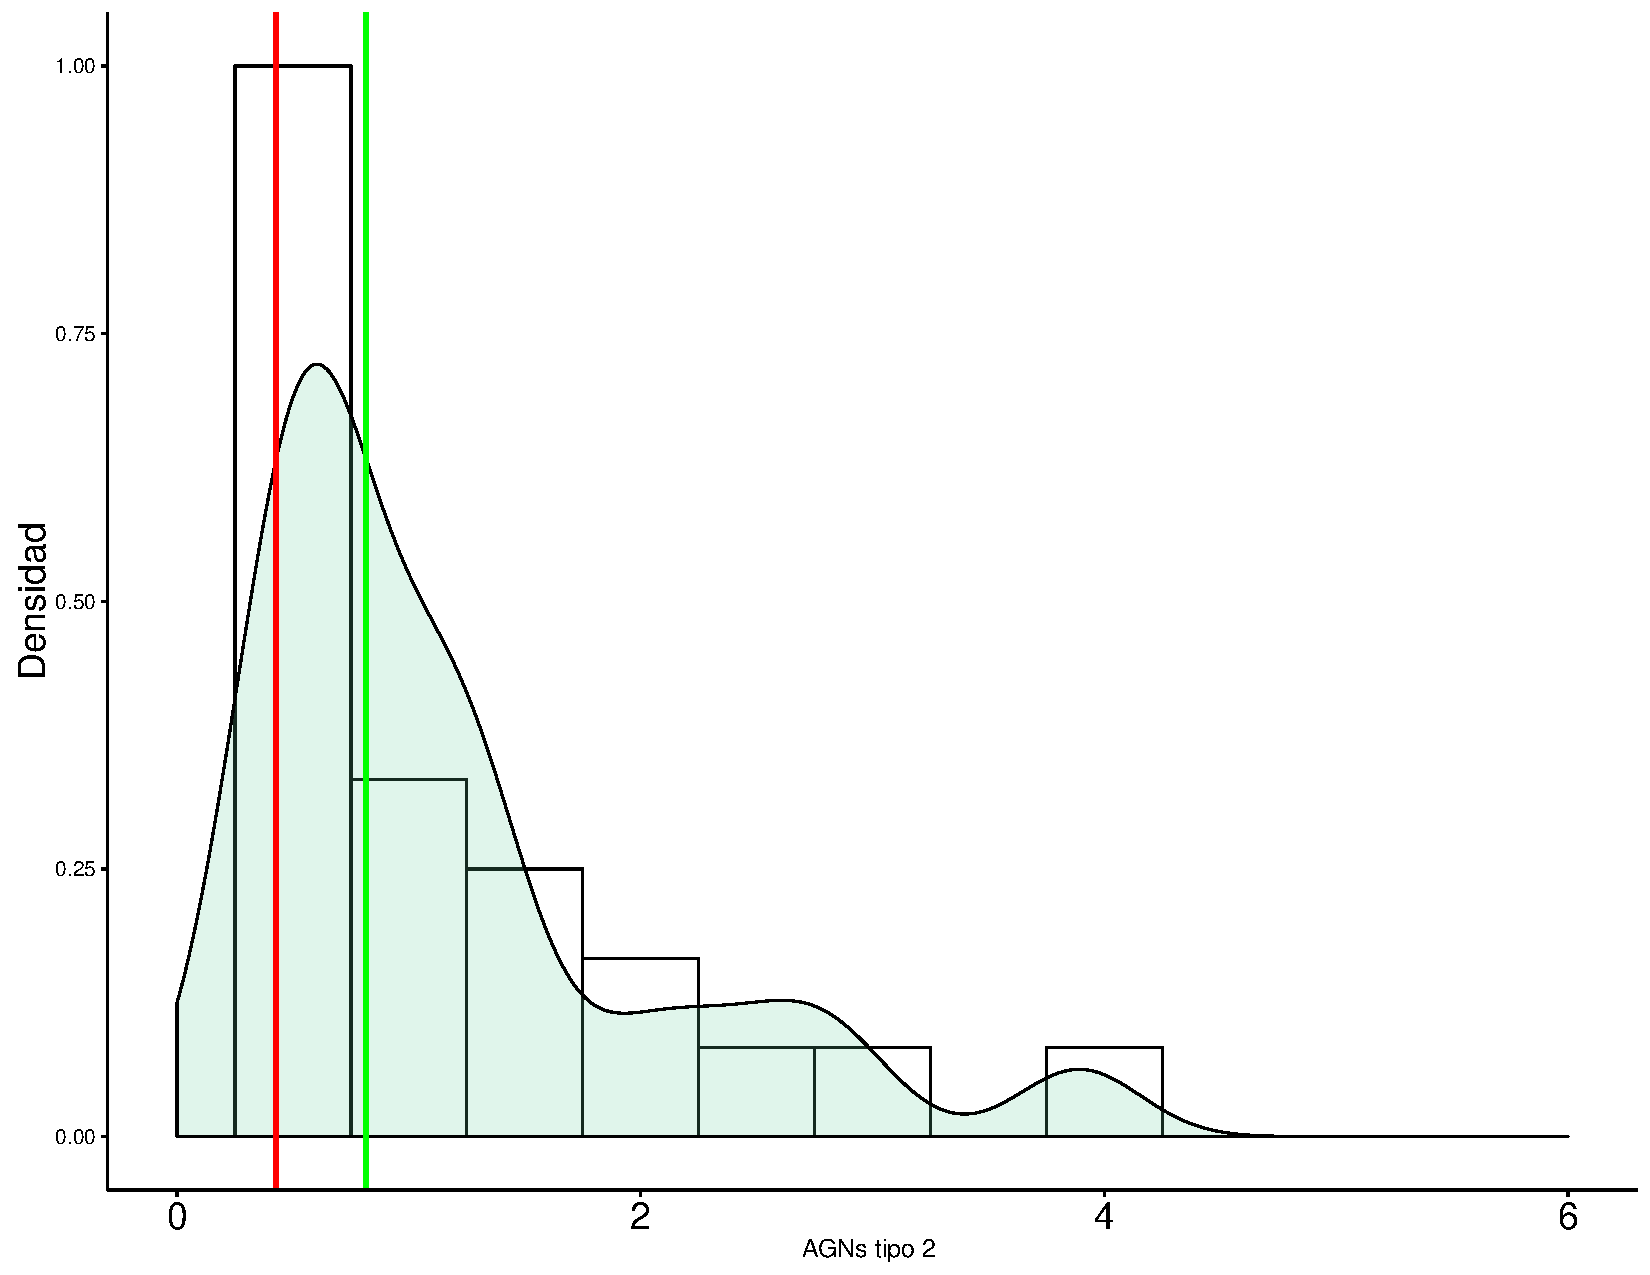
\includegraphics[width=90mm]{chi_agns.pdf}
\caption[Distribuciones $\chi^2_{\nu}$ para AGNs tipo 2] {Distribuciones $\chi^{2}_{\nu}$ los AGNs tipo 2 en la muestra. La línea roja corresponde a la $\chi^{2}_{\nu}$ de UGC11680 con respecto a la categoría señalada. La línea verde corresponde a la media de la distribución para esta categoría}
\label{ensamblaje_cara}
\end{figure}


\begin{figure}
  \centering
    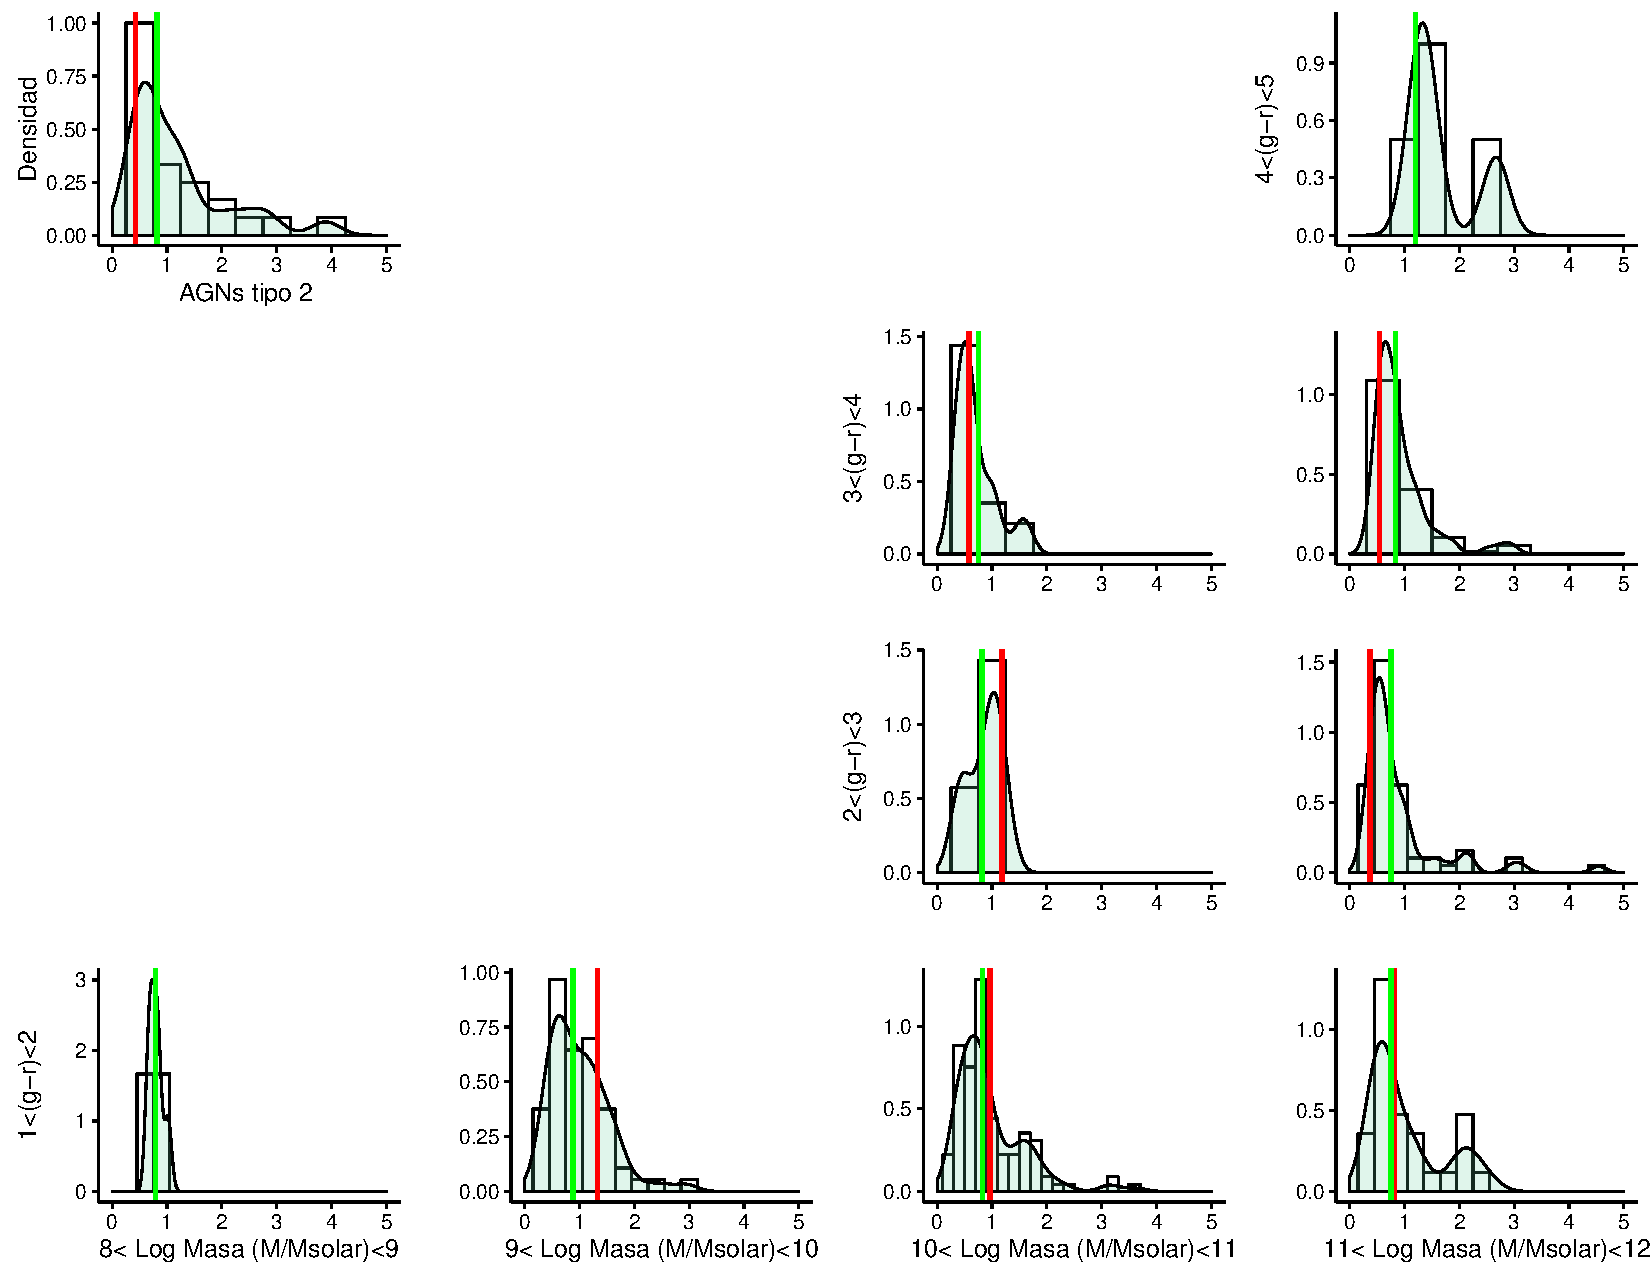
\includegraphics[scale=0.5]{exp_chi_perl.pdf}
  \caption[Diagrama de distribuciones $\chi^{2}_{\nu}$ en Color-Masa ]{Representación del Diagrama Color-Masa  con las distribuciones $\chi^2_{\nu}$ pertenecientes a su intervalo correspondiente.Cada distribución $\chi^2_{\nu}$ de la muestra de  \textbf{CALIFA}. La línea roja es la $\chi^2_{\nu}$ de UGC11680 para cada una de su categoría y la línea verde corresponde a la media de las distribuciones.En la esquina superior izquierda se colocaron las $\chi^2_{\nu}$ de los AGNs tipo 2 como referencia referencia }
  \label{chi_todos_mean}
\end{figure}




\begin{equation}
\chi^{2}_{\nu} = \frac{1}{2} \sum_{t=1}^{n_t} \sum_{R=1}^{n_R}  \frac{ \left[SFH_{data}(t,R)- \left <SFH_{cat}(t,R) \right > \right]^2}{\sigma(t,R)_{cat}^2}
\end{equation}

\bigskip

\noindent Donde $n_t$ , $n_R$ son las dimensiones temporales y radiales respectivamente, $SFH_{data}(t,R)$ es el flujo de la imagen a comparar ($\Sigma_{*}$, para los mapas $SFH$); $\left <SFH_{cat}(t,R)\right >$ es el mapa promedio definido anteriormente y finalmente  $\sigma(t,R)_{cat}^2$ es el mapa de dispersión de los datos por cada categoría definido como

\begin{equation}
\sigma(t,R)^2= \frac{1}{m-1} \sum_{i=1}^{m} \left[SFH_{i}(t,R)- \left <SFH_{cat}(t,R) \right > \right]^2.
\end{equation}


\bigskip

\noindent Una vez definido el parámetro $\chi^{2}_{\nu}$ lo usamos para definirlo en cada galaxia de la muestra  con respecto al promedio de su categoría. La $\chi^{2}_{\nu}$ de UGC11680 se colocó por separado para fines comparativos, así obtenemos 575 $\chi^{2}_{\nu}$ y 25 para la categoría de los AGNs. Estas $\chi^{2}_{\nu}$ se usan para su distribución con la categoría correspondiente y estas se muestran en la Figura \ref{ensamblaje_cara} que es el caso de la distribución de las $\chi^{2}_{\nu}$ para los AGNs tipo 2 y donde la $\chi^{2}_{\nu}$ de UGC11680 se muestra con una linea roja y la media con una línea verde, para comparaciones posteriores.

\bigskip

\noindent Estas distribuciones pueden ser también mostradas construyendo un diagrama que simule el diagrama color-masa para galaxias, como  se muestran en la Figura \ref{chi_todos_mean}, donde como en el caso anterior, se representa la $\chi^{2}_{\nu}$ de UGC11680 con una línea roja y la media con una línea verde. En la esquina superior izquierda colocamos la distribución de los AGNs para referencia. Nótese que se obtuvieron distribuciones  asimétricas, lo que concuerda con la distribución típica de una $\chi^{2}$ reducida.

\begin{figure}
  \centering
    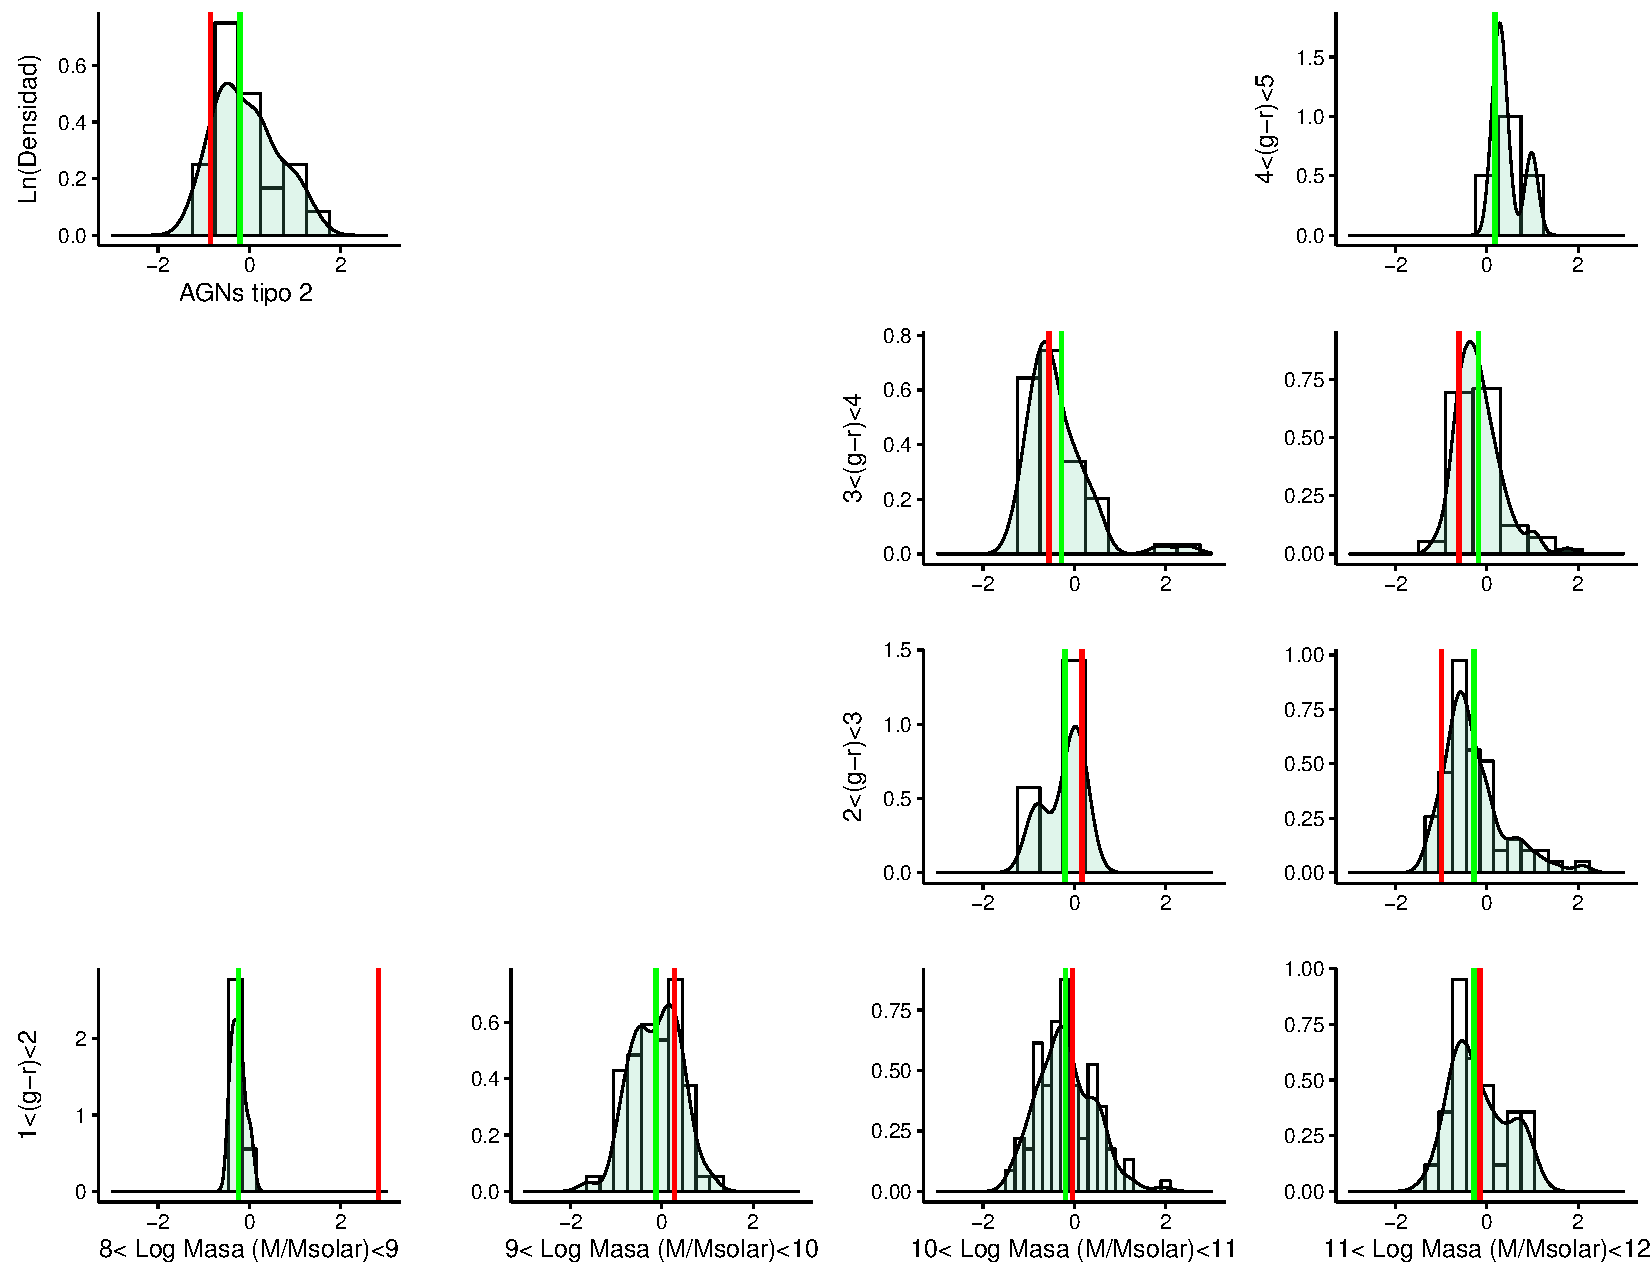
\includegraphics[scale=0.5]{log_chi_perl.pdf}
  \caption[Diagrama de distribuciones Log-Normal para $\chi^{2}_{\nu}$ en Color-Masa]{Diagrama Log-Normal para las distribuciones Color-Masa  de las $\chi^2_{\nu}$ pertenecientes a su intervalo correspondiente. La línea roja es la Log-Normal $\chi^2_{\nu}$ de UGC11680 para cada una de su categoría y la línea verde corresponde a la media Log-Normal de las distribuciones.En la esquina superior izquierda se colocaron las Log-Normal $\chi^2_{\nu}$ para los AGNs tipo 2  para referencia }
  \label{chi_todos_log}
\end{figure}



\subsection{Ajuste de $\chi^2_{UGC11680}$ con respecto a las Distribuciones Categóricas}


\noindent Como se mencionó anteriormente, la idea principal es buscar un ajuste de UGC11680 con respecto a cada $\chi^2_{\nu}$ de las categorías de la muestra tal que nos diga a que categoría se ``parece'' o ajusta mejor en su historia de formación estelar. Esto implicaría historias de formación estelar comunes  para las categorías que ajustan mejor con nuestra galaxia.  Observamos entonces que en la Figura \ref{chi_todos_mean} al ser $\chi^2_{\nu}$ una distribución no simétrica por construcción, el máximo no coincide necesariamente con la media de los datos. Además, la dispersión es un valor que oscila para cada categoría, por lo que para definir un ajuste que dependa de la media y su dispersión, consideramos que la distribución $\chi^2_{\nu}$ que construimos es una aproximación a la distribución Log-Normal, por lo que a todos los valores $\chi^{2}_{\nu}$  los escalamos tomando el logaritmo a cada uno de ellos. El resultado de esta distribuciones logarítmicas se muestran en la Figura \ref{chi_todos_log}, donde la $\chi^{2}_{\nu}$ de UGC11680  es la línea roja y la media la linea verde. Los rangos de las distribuciones son las mismos para todas las figuras. Debido a la transformación, obtenemos una distribución cuasi-Gaussiana para cada categoría y esto ya nos permitirá definir un ajuste con respecto a valores conocidos de una distribución normal. Teniendo en cuenta esto, para determinar a que categoría se asemeja más el mapa $SFH$ de UGC11680 comparamos ahora los valores de $\chi^{2}_{\nu}$ en escala logarítmica con respecto a la $\chi^2_{\nu}$ de UGC11680, normalizados a la dispersión logarítmica de los datos por categoría. Definimos entonces el ajuste de UGC11680 con respecto a estas como


\begin{equation}
AJ(\chi^2_{\nu})= \frac{ \ln(\chi^2_{UGC11680})  -  < ln (\chi^2_{cat})>} {\sigma_{\ln(\chi^2_{cat})}}
\end{equation}



\bigskip

\noindent Para obtener este valor de $AJ(\chi^2_{\nu})$ se iteró 3 veces con 2 lenguajes de programación diferentes (PERL y PYTHON)  para mejores resultados y estos se muestran en la tabla \ref{estadistica}

\begin{figure}[htbp]
\centering
\subfigure{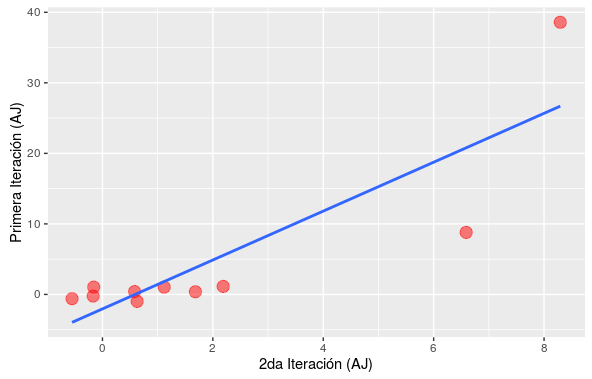
\includegraphics[width=70mm]{primer_scatter.png}}
\subfigure{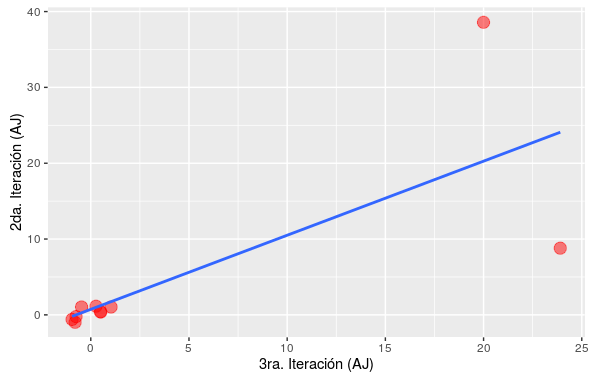
\includegraphics[width=70mm]{segundo_scatter.png}}
\caption[Correlación entre ajuster]{Correlación entre las diferentes iteraciones para calcular el valor de ajuste $|AJ(\chi^{2}_{\nu})|$ para la $\chi^{2}_{\nu}$ de UGC11680 con respecto a los promedios de cada categoría. Nótese que la dispersión para los valores mas grandes con respecto a la galaxia UGC11680 corresponden también a una $\chi^{2}_{\nu}$ grande, por lo que estos valores son de poca importancia estadística dentro del análisis.}
\label{correlacion}
\end{figure}


\begin{table}[!ht]
\centering
\begin{tabular}{||c | c | c | c ||}
\hline
\hline
Categoría & Primera Iteración &  2da. Iteración & 3era. Iteración \\
\hline
\hline
$(8<M_{\odot}<9)_{1<g-r<2}$  &  8.293 &  38.58 &  19.997 \\
$(9<M_{\odot}<10)_{1<g-r<2}$ &  1.118 & 1.035 &  1.032 \\
$(10<M_{\odot}<11)_{1<g-r<2}$ & 0.583 & 0.408 & 0.495 \\
$(10<M_{\odot}<11)_{2<g-r<3}$ & 1.684 &  0.378 & 0.508\\
$(10<M_{\odot}<11)_{3<g-r<4} $ & 0.167 & 0.226 &  0.749 \\
$(11<M_{\odot}<12)_{1<g-r<2} $ & 2.187 &  1.139 &  0.266 \\
$(11<M_{\odot}<12)_{2<g-r<3} $  & 0.628 &  0.986 & 0.798  \\
$(11<M_{\odot}<12)_{3<g-r<4} $  & 0.550 &  0.599 & 0.953 \\
$(11<M_{\odot}<12)_{4<g-r<5}$ & 6.589 & 8.792 &  23.90 \\
                        AGNs  & 0.158 & 1.037  & 0.469\\
\hline
\hline
\end{tabular}
\caption{Valores para el ajuste $AJ(\chi^2_{\nu})$ en tres diferentes iteraciones, utilizando mismo algoritmo pero en dos lenguajes de programación diferentes (PERL y PITHON). Nótese que la única discrepancia entre los diferentes ajustes corresponde a las categorías que contienen menos objetos. LA primera iteración corresponde a la reducción 1.5 de los datos de \textbf{CALIFA} y para los DR2 de los mismos. Las iteraciones 2 y 3 corresponden a la versión 2.2 de los datos, DR3, usando PERL PDL para la segunda  y PYTHON NumPy para la tercera. }
\label{estadistica}
\end{table}

\bigskip

\noindent Observando los valores de la tabla \ref{estadistica} aunque son del orden entre las diferentes categorías lo que se muestra en la figura \ref{correlacion} existe una cierta discrepancia entre los datos que se obtienen; esto se debe probablemente a la naturaleza de la definición para el ajuste $|AJ(\chi^{2}_{\nu})|$ así como la sensibilidad de los diferentes algoritmos en el truncamiento de valores cuando se define el logaritmo natural en diferentes lenguajes de programación. Obsérvese que los valores que más se dispersan en las Figuras en \ref{correlacion} corresponde a las categorías que contienen menos objetos y esto en sí mismo podría ser la causa de la dispersión. Sin embargo, esta discrepancia esta dentro del orden de los valores que se obtienen para cada ajuste, además de que la $\chi^{2}_{\nu}$ de UGC11680 esta muy alejada en realidad de la media de su distribución para las categorías con menos objetos, por lo que en si mismo, este ajuste no es tan significativo como los obtenidos para las otras categorías.


\bigskip

\noindent Técnicamente hablando, no podemos afirmar cual valor es el correcto para las iteraciones del ajuste de las $\chi^{2}_{\nu}$ de las historias de formación estelar, por lo que para obtener  el valor más cercano que nos indique el número más cercano para comparar  estas historia de formación de UGC11680 con respecto a sus diferentes categorías, usamos el valor medio de cada ajuste obtenido, generando así el que mejor se acerca a la $\chi^{2}_{\nu}$ de la historia de formación para la galaxia en cuestión. Estos valores se muestran para las distribuciones $\chi^{2}_{\nu}$ para cada categoría estudiada en la Tabla \ref{tab_LN2}. Los resultados se colocaron en orden descendente con respecto a $|AJ(\chi^2_{\nu})|$, de menor a mayor, donde el valor menor corresponde a un mejor ajuste de UGC11680 con respecto a la categoría indicada.



\bigskip

\begin{table}[!ht]
\centering
\begin{tabular}{||c | c | c | c | c||}
\hline
\hline
Categoría & $ \sigma_{\ln \chi^{2}_{\nu}}$ & $ <\ln(\chi^2_{cat})> $ & $\ln \chi^{2}_{UGC11680}$ & $|AJ(\chi^{2}_{\nu})|$ \\
\hline
\hline







$(10< \log M_{\odot}< 11)_{3<g-r<4}$  & 0.712  & -0.283  &-0.551  & 0.226 \\
                                  AGNs  & 0.540 & -0.205 & 0.445  & 0.469 \\
$(10< \log M_{\odot}< 11)_{1<g-r<2}$  & 0.608 & -0.192 & -0.035  & 0.495 \\
$(10< \log M_{\odot}< 12)_{2<g-r<3}$  & 0.596 & -0.205 & 0.058  & 0.508 \\
$(11< \log M_{\odot}< 12)_{3<g-r<4}$  & 0.501 & -0.181  & -0.612 & 0.599 \\
$(11<  \log M_{\odot}< 12)_{2<g-r<3}$ & 0.648 & -0.278  & -0.988  & 0.798 \\
$(9< \log M_{\odot}< 10)_{1<g-r<2}$   & 0.528 & -0.129 & 0.282  & 1.035 \\
$(11< \log M_{\odot}< 12)_{1<g-r<2}$  & 0.606 & -0.278 & -0.199  & 1.139 \\
$(11< \log  M_{\odot}< 12)_{4<g-r<5}$  & 0.503 & 0.183 & 11.55 & 8.792 \\
$(8< \log M_{\odot}< 9)_{1<g-r<2}$    & 0.157  & -0.237 & 2.83 & 19.997 \\



\hline
\hline
\end{tabular}
\caption{Tabla de los valores estadísticos para la comparación de UGC11680 con respecto a las categorías que se indican, comenzando con la dispersión, la media el valor $\chi^{2}_{\nu}$ de UGC11680 y finalmente el ajuste de su valor $\chi^{2}_{\nu}$ con respecto a cada una de ellas. El orden de los valores esta dado por $|AJ(\chi^{2}_{\nu})|$ del  menor a mayor que corresponderían al grado de mejor a menor ajuste de UGC11680 con respecto a las categorías indicadas. Todos los datos estadísticos se encuentran en escala logarítmica}
\label{tab_LN2}                              %etiqueta para referencia
\end{table}

\bigskip


\noindent Antes de interpretar los valores obtenidos, debemos recordar que estamos comparando historias de formación estelar por medio del mapa $SFH$, por lo que un parecido entre promedios por categorías y UGC11680 es un parecido en este contexto, de como los promedios de historia de formación estelar estudiadas  de la muestra de \textbf{CALIFA} y separadas por categorías coinciden con la galaxia espiral roja. De esta forma, con los valores de la tabla podemos Observamos el orden en que ajusto mejor la galaxia UGC11680:


\begin{itemize}

\item Ell mejor ajuste resulto ser para las galaxias rojas y masivas correspondientes a la categoría a la que pertenece UGC11680 $\sim 10^{10} \log M_{\odot}$ , $3<\text{color}<4$, esto nos indicaría que UGC11680 ajusta en su historia de formación estelar con las de su categoría.


\item  El segundo mejor ajuste corresponde a el grupo de los AGNs. Esto nos indicaría que el AGN de alguna forma influye o altera la formación estelar, al menos para las galaxias de la muestra.

\item  El tercer y cuarto mejor ajuste corresponde al grupo de  de galaxias  de masa intermedia, que se encuentran en el valle verde ($10< \log M_{\odot} < 11$ color $1<g-r<2$) y ($10< \log M_{\odot}< 11$ color $2<g-r<3$). Este resultado es interesante ya que la galaxia aun siendo de color rojo en el óptico, coincide en formación estelar con las galaxias en la llamada zona de transición.

\item Por último, los últimos mejores ajustes corresponden a las galaxias más masivas y rojas masivas  comenzando por las mas rojas ($10< \log M_{\odot}< 11)$ color $3<g-r<4$) seguidas por las menos rojas que las anteriores ($11< \log M_{\odot}< 12$ color $2<g-r<3$).


\end{itemize}

\bigskip


\noindent Los demás valores del ajuste corresponden a las galaxias que menos encajan con UGC11680, que en general son las galaxias que están en la nube azul, ya sean masivas o no, así como las galaxias mas masivas y rojas de toda la muestra, que aunque contiene pocos objetos, la discrepancia es demasiada como para ser estadísticamente relevante. Podríamos decir que el ajuste en historia de formación estelar  de UGC11680 coincide con las de su categoría, las galaxias de masa intermedia en el rango del color rojo, los AGNs tipo 2, las galaxias de masa intermedia en la zona de transición conocida como el valle verde y finalmente a las galaxias masivas en los límites entre la secuencia roja y la zona de transición. Los demás ajustes se alejan de un valor relevante para el estudio de la galaxia por lo que su valor no nos indican alguna semejanza en historia de formación estelar para que pueda considerarse como un ``parecido'' dentro de la definición que hemos estado manejando. Estos resultados ya nos indican que UGC11680 es una galaxias peculiar, en donde el AGN y su masa juegan un papel importante y que fueron determinantes para detener la formación estelar desde dentro hacia afuera, empezando a épocas cosmológicas tempranas ($\sim$ 9 Gyrs).









